%!TEX root = ../Base.tex


%*****************************************
\chapter{Modelos de Márkov}\label{ch:chap2}
%*****************************************

\epigraphhead[70]{
\epigraph{Essentially, all models are wrong, but some are useful.}
         {George E. P. Box}}

Como ya se mencionó en la Introducción, se debe proponer un modelo acústico o generativo, que será la forma en que entenderemos y trataremos de abstraer la conversación o diálogo, de acuerdo a las características que nos interesan recuperar.

Puesto que lo que nos interesa principalmente es identificar a las diferentes personas que participan en una conversación, nuestro modelo se deberá parametrizar de forma que logre capturar las características esenciales en la conversación; así como no tomar en cuenta información que no nos sea de utilidad para esta tarea, como por ejemplo, qué es lo que se está diciendo.

En aprendizaje máquina, por modelo generativo se entiende un modelo probabilístico para generar datos aleatoriamente que correspondan a la naturaleza de un cierto conjunto de datos que tengamos.

Al proponer un modelo generativo, se busca representar y de forma concisa poder parametrizar un fenómeno o situación de la que se obtuvieron los datos.
Cuando los datos son secuenciales, se suelen agrupar en dos tipos, de acuerdo a las características de la distribución que los generó: distribuciones estacionarias y distribuciones no estacionarias.

En el caso de secuencias de datos estacionarias, se considera que los datos \textit{evolucionan} a través del tiempo, pero la distribución a partir de la cuál fueron generados permanece igual; mientras que para el caso de datos no estacionarios, su distribución generativa varía también según pasa el tiempo.

Para el problema de \sd, consideraremos que los datos son estacionarios; es decir, supondremos que su distribución generativa no cambia. Para resolver nuestro problema entonces trataremos a partir de los datos ajustar una distribución inicial e inferir sus parámetros correspondientes.

Este tipo de abstracción, permiten modelar una gran cantidad de situaciones, en las que se tienen observaciones de acuerdo al tiempo y se quiere predecir el siguiente valor en la serie, dadas la observaciones que se tienen hasta el momento.

Comúnmente se suelen considerar únicamente las observaciones más recientes, pues son las que pudiéramos pensar son más informativas para la predicción; además de que al asumir que las predicciones de nuevos datos sólo dependen de las últimas observaciones, nos permite simplificar mucho el modelo de la distribución generativa.

Para trabajar con este tipo de datos, se puede usar entonces un modelo de Márkov que es un proceso aleatorio muy trabajado en la teoría de probabilidad, que incorpora una cantidad mínima de memoria, sin necesariamente llegar a ser un proceso sin memoria.

Se puede pensar como una red bayesiana en la que se asume la independecia de las variables aleatorias que corresponden a las predicciones futuras con todas las observaciones excepto las últimas (i.e. el futuro es independiente del pasado, dado el presente).

\section{Cadena de Markov}

\graffito{Se entiende por v.a. i.i.d aquellas que son independientes entre sí y que fueron muestreadas de la misma distribución}

El modelo generativo más sencillo que se podría pensar, es considerar que todas las observaciones son variables aleatorias independientes e idénticas distribuidas (v.a. i.i.d) cuyo modelo gráfico se muestra en la \autoref{fig:mod_iid}.

\begin{figure}[bt]
        \myfloatalign
        {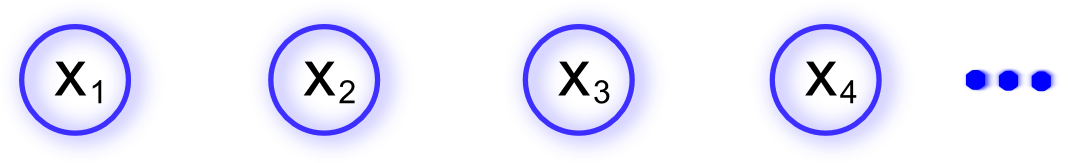
\includegraphics[width=0.6\linewidth]{gfx/chap2/mod-iid}}        
        \caption{Observaciones independientes e idénticamente distribuidas.}
        \label{fig:mod_iid}
\end{figure}

Al asumir que no hay ninguna dependencia entre los datos, sin embargo, se pierde la información relativa al orden en que se fueron dando estas observaciones; situación que en muchos casos nos interesa conservar.

Si se tiene un conjunto $N$ de observaciones $\mb{X} = \lbrace x_1, ..., x_n \rbrace$, y se asume que son i.i.d, la distribución conjunta de la secuencia de datos se puede escribir como sigue:
\begin{equation}
\label{eqn:2-1}
p(x_1, ..., x_N) ~=~ \prod_{n=1}^N p(x_n)
\end{equation}

En cambio, para expresar la dependencia entre un grupo de observaciones secuenciales, se puede utilizar un modelo probabilístico llamado \textit{modelo o cadena de Markov}. Si por ejemplo, se considera que cada variable depende de todas las observaciones anteriores, entonces usando el teorema de bayes
\graffito{Del teorema de Bayes se tiene la siguiente expresión
$${P(A \,|\, B) = \frac{P(B \,|\,A) P(A)}{P(B)}}$$ } 
se puede escribir la distribución conjunta de las observaciones de la siguiente manera:
\begin{equation}
\label{eqn:2-2}
p(x_1, ..., x_N) ~=~ \prod_{n=1}^N p(x_n \,|\, x_1, ..., x_{n-1}).
\end{equation}

Ahora, si se asume que cada $x_n$ es independiente de las observaciones anteriores excepto de la observación anterior $x_{n-1}$, se tiene que la distribución conjunta se puede escribir de forma más sencilla utilizando el teorema de separación D \footnote{Ver anexo}, puesto que 
\begin{equation}
\label{eqn:2-3}
p(x_n \,|\, x_1, ..., x_{n-1}) ~=~ p(x_n \,|\, x_{n-1})
\end{equation}

A este modelo probabilístico se le conoce como cadena de Márkov de primer orden y la probabilidad conjunta de las observaciones está dada por:
\begin{equation}
\label{eqn:2-4}
p(x_1, ..., x_N) ~=~ p(x_1) \prod_{n=2}^N p(x_n \,|\, x_{n-1}).
\end{equation}
mientras que su modelo gráfico corresponde a la \autoref{fig:mod_mm1}
\begin{figure}[bt]
        \myfloatalign
        {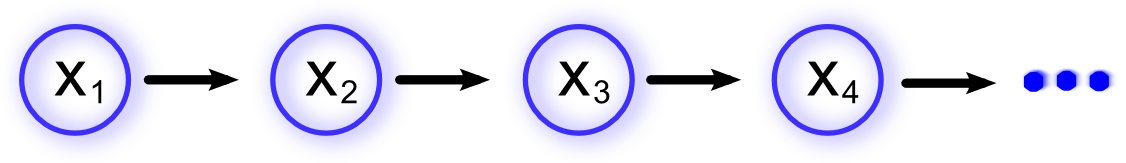
\includegraphics[width=0.6\linewidth]{gfx/chap2/mod-mm1}}
        \caption{Modelo de Márkov de primer orden.}
        \label{fig:mod_mm1}
\end{figure}

Aunque el modelo es mucho más general, puede que se necesite representar de forma más fuerte la dependencia con las osbervaciones anteriores, por lo que se pueden usar cadenas de Márkov de órdenes superiores.

Al caso en el que $x_n$ dependa de las dos observaciones previas se le conoce como cadena de Márkov de segundo orden; y siguiendo el mismo proceso, la distribución conjunta de las observaciones se puede escribir como 
\begin{equation}
\label{eqn:2-5}
p(x_1, ..., x_N) ~=~ p(x_1) \cdot p(x_2 \,|\, x_1) 
        \prod_{n=3}^N p(x_n \,|\, x_{n-1}, x_{n-2})
\end{equation}
puesto que se tiene que $x_n \perp x_1, ..., x_{n-3} \,|\, x_{n-1}, x_{n-2}$.

En este caso su modelo gráfico correspondiente es la \autoref{fig:mod_mm2}, en el que se puede observar la dependencia de una $x_n$ en específico únicamente con sus dos observaciones anteriores.

\begin{figure}[bt]
        \myfloatalign
        {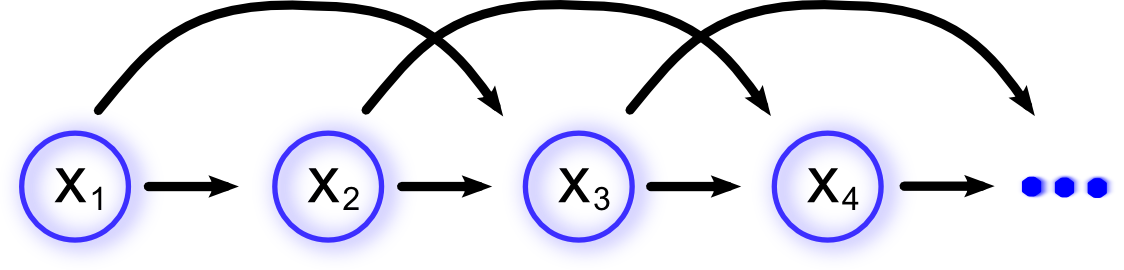
\includegraphics[width=0.6\linewidth]{gfx/chap2/mod-mm2}}
        \caption{Modelo de Márkov de segundo orden.}
        \label{fig:mod_mm2}
\end{figure}

Se puede generalizar entonces para cualquier $M$ un modelo de Márkov de $M$-ésimo orden, aunque al considerar demasiados estados previos se puede complicar de más el modelo; pues el número de parámetros implicados aumenta de forma exponencial al orden del modelo de Márkov.

Para evitar que el modelo se vuelva demasiado complejo, así como para no hacer alguna suposición a priori sobre cuál es el orden es del modelo generativo, se puede introducir una variable oculta, que permita cambiar el planteamiento del modelo. 

Se considera entonces una variable latente $z_n$ correspondiente a cada  observación $x_n$, y entonces el conjunto de variables latentes forman una cadena de Márkov, como se muestra en la \autoref{fig:mod_hmm1}.

Se asumirá entonces 
\begin{equation}
\label{eqn:2-6}
z_{n+1} \perp z_{n-1} \,|\, z_{n}
\end{equation}

Y entonces, usando la regla de la cadena, la distribución conjunta para este modelo es la siguiente: 
\begin{equation}
\label{eqn:2-7}
p(x_1, ..., x_N, z_1, ..., z_N) ~=~ 
        p(z_1) \left [ \prod_{n=2}^N p(z_n \,|\, z_{n-1}) \right ] 
\prod_{n=1}^N p(x_n \,|\, z_{n}).
\end{equation}

\begin{figure}[hbt]
        \myfloatalign
        {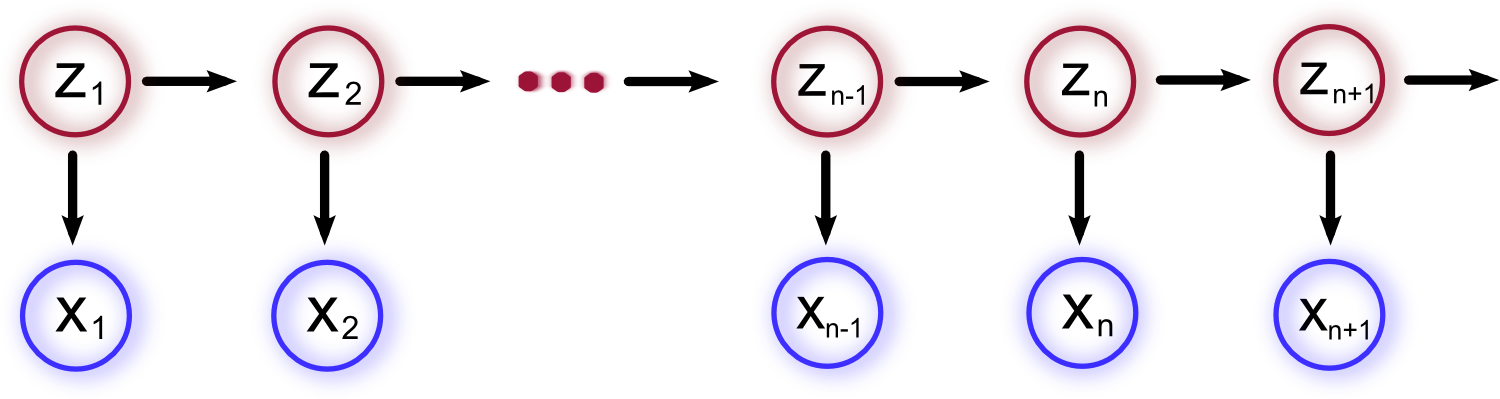
\includegraphics[width=0.8\linewidth]{gfx/chap2/mod-hmm1}}
        \caption{Modelo oculto de Márkov.}
        \label{fig:mod_hmm1}
\end{figure}

Para éste último modelo gráfico, si las variables latentes son discretas, entonces se le conoce como Modelo oculto de Márkov o HMM (\textit{Hidden Markov Model}), y es justo el modelo que se utilizará para resolver la tarea de \sd.

\section{Cadena oculta de Márkov}

Una cadena oculta de Márkov, sigue siendo entonces un modelo para datos secuenciales, en los que además se introduce el concepto de una variable oculta de la cual dependen las observaciones que se tienen; y de forma más especifica, esta variable oculta es discreta. 

Usando un HMM entonces podemos modelar un proceso bivariado discreto en el tiempo, con ciertas propiedades interesantes que se mencionarán más adelante.

Nuestro modelo HMM, se puede pensar como una mezcla de distribuciones en la que la densidad tiene un distribución dada por $p(x|z)$, es decir, la mezcla de los componentes está dada por las observaciones previas.

Se puede considerar entonces, que cada variable latente $z_n$ tendrá una distribución multinomial discreta, que indicará cuál componente de la mezcla de distribuciones es la que ha generado la observación $x_n$. Para ésto, se usará la notación \unk, que corresponde a un conjunto de variables indicador $z_{nk} \in \lbrace 0, 1 \rbrace$, donde $k = 1, ..., K$ señalando cuál de las $K$ distribuciones generó a la variable $x_n$, \ie, si el componente generador de $x_n$ fue la $k$-ésima mezcla, entonces $z_{nk} = 1$ y $z_{nj} = 0$ para todo $j \neq k$.

Ahora, se tiene que cada variable $z_n$ depende únicamente de $z_{n-1}$, y puesto que las variables latente son vectores binarios de $K$ dimensiones, entonces se tendría que la probabilidad condicional de $z_n \,|\, z_{n-1}$ se puede representar mediante una tabla o matriz, que se denotará como $\mb{A}$, y será referida como \textit{matriz de probabilidades de transición}. 

Los componentes de la matriz de transición se definen tal que $A_{jk} \equiv p(z_{nk} = 1 \,|\,  z_{n-1, j} = 1)$, y puesto que son probabilidades, se cumple que $0 \leq A_{jk} \leq 1$ además de que $\sum_k A_{jk} = 1$. Considerando estas restricciones, entonces la matriz $\mb{A}$ tiene $K (K-1)$ parámetros independientes.

Se puede escribir entonces la probabilidad condicional de una variable latente $z_n$ dada la anterior variable latente $z_{n-1}$ de la siguiente forma: 
\begin{equation}
\label{eqn:2-8}
p(z_n \,|\, z_{n-1}, \mb{A}) = \prod_{k=1}^K \prod_{j=1}^K A_{jk}^{z_{n-1, j} 
        \cdot z_{nk}}
\end{equation}

Además, se tiene que considerar la variable latente inicial $z_1$, puesto que ésta no tiene una variable latente anterior, la \autoref{eqn:2-7} no aplica; por lo que entonces la probabilidad marginal de $z_1$ está representada por un vector de probabilidades $\pi$ tal que $\pi_k \equiv p(z_{1k})$, por lo que se puede reescribir como sigue: 
\begin{equation}
p(z_1 \,|\, \pi) = \prod_{k=1}^K \pi_k^{z_{1k}}
\label{eqn:2-9}
\end{equation}
y además se cumple que $\sum_k \pi_k = 1$ por definición.

La matriz de transición también se puede llegar a representar como un grafo dirigido, si se consideran las entradas de la matriz $\mb{A}$ como los pesos de las aristas, y los nodos son cada uno de los posibles $K$ estados. Por ejemplo, para el caso de una variable latente de $K = 3$ estados, se tendría el grafo de la \autoref{fig:mod_hmm2}.

\begin{figure}[hbt]
        \myfloatalign
        {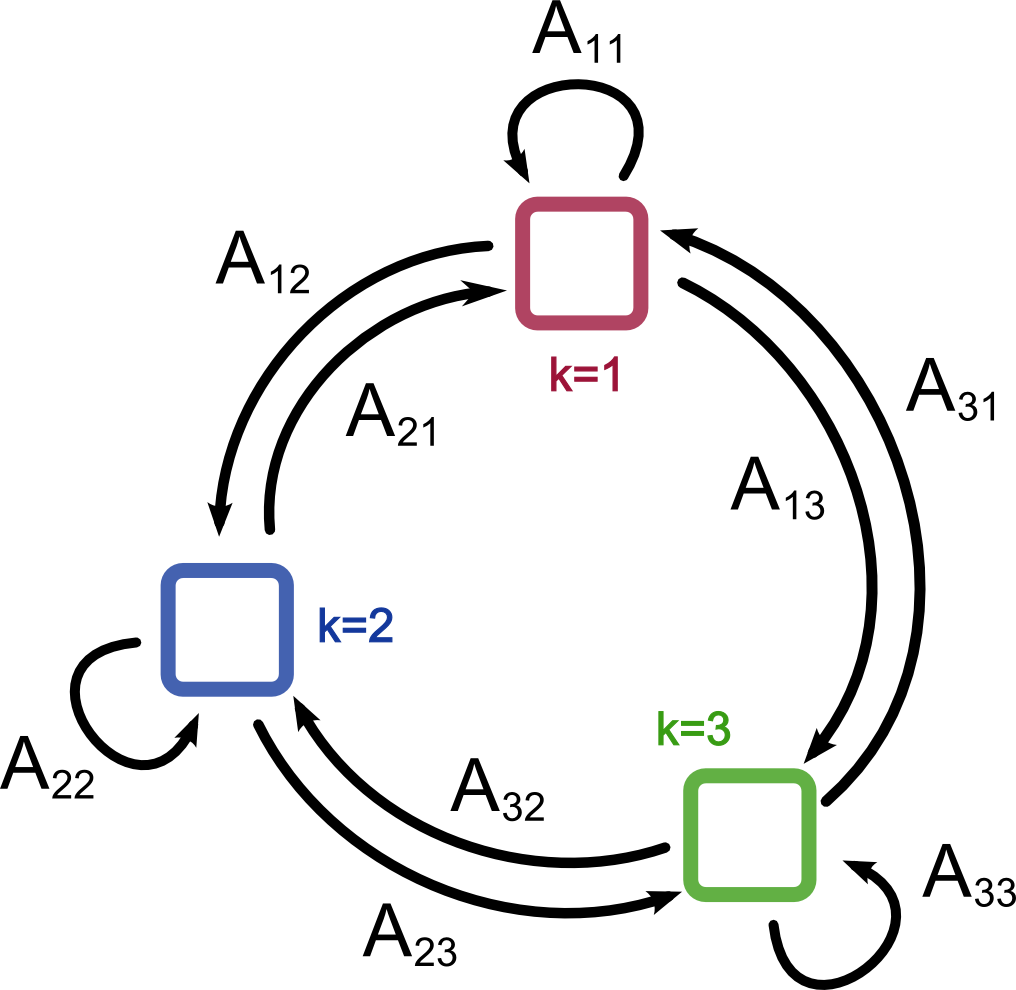
\includegraphics[width=0.4\linewidth]{gfx/chap2/mod-hmm2}}
        \caption{Matriz de transición de modelo oculto de Márkov (grafo).}
        \label{fig:mod_hmm2}
\end{figure}

De la misma manera, el grafo correspondiente a la matriz de transición, se puede representar como una rejilla a través del tiempo, en la que se mantienen los vértices y aristas del grafo, pero además se introduce la noción del tiempo. Como se observa en la \autoref{fig:mod_hmm3} 

\begin{figure}[hbt]
        \myfloatalign
        {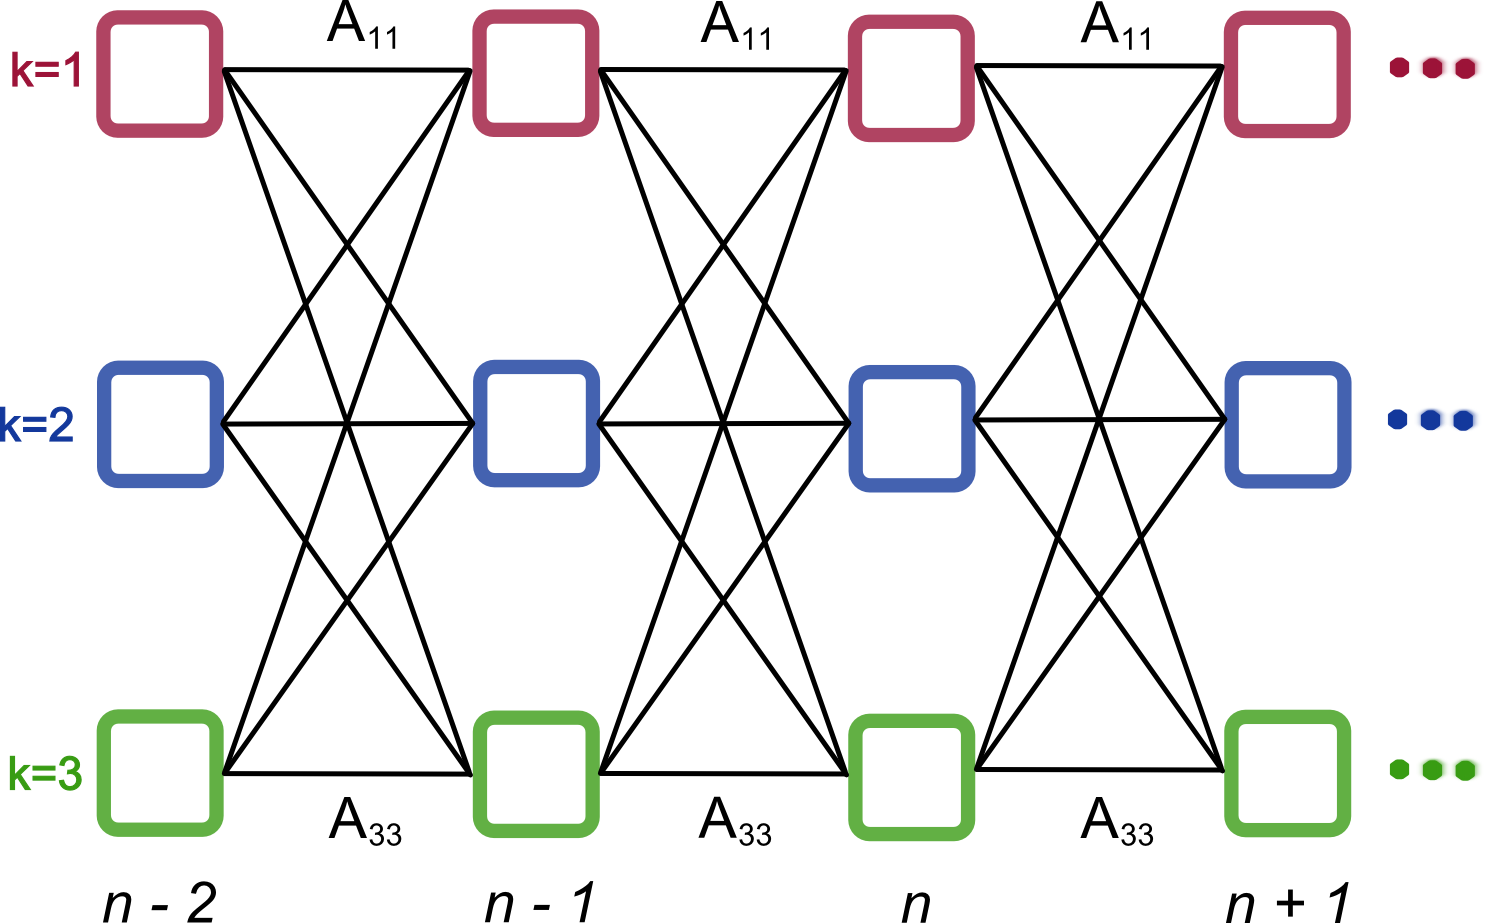
\includegraphics[width=0.63\linewidth]{gfx/chap2/mod-hmm3}}
        \caption{Matriz de transición de modelo oculto de Márkov (rejilla).}
        \label{fig:mod_hmm3}
\end{figure}

Por último, para completar el modelo se tiene que considerar además la distribución condicional de las variables observadas, es decir $p(x_n \,|\, z_n, \phi)$ donde $\phi$ es un conjunto de parámetros específicos a la distribución de $x$. Se les conoce como probabilidades de emisión, y puede ser tanto una distribución discreta como una continua. Para el caso en que la probabilidad de emisión esté dada por una distribución discreta, entonces se tendrá una tabla de probabilidades.

Para calcular entonces esta probabilidad de emisión, se tiene tanto $z_n$ como unos parámetros $\phi$ dados, por lo que entonces se tienen un vector de $K$ valores para cada uno de los posibles estados del vector indicador $z_n$.

Se puede escribir entonces la probabilidad de emisión como sigue:
\begin{equation}
p(x_n \,|\, z_n, \phi) = \prod_{k=1}^K p(x_n \,|\, \phi_k) ^ {z_{nk}}
\label{eqn:2-10}
\end{equation}
y entonces la probabilidad conjunta quedaría definida de la siguiente manera:
\begin{equation}
p(\mb{X}, \mb{Z} \,|\, \theta) 
= p(z_1 \,|\, \pi) \left[ \prod_{n=2}^N p(z_n \,|\, z_{n-1}, \mb{A}) \right]
        \prod_{n=1}^N p(x_n \,|\, z_n, \phi)
\label{eqn:2-11}
\end{equation}
donde $\mb{X} = \lbrace x_1, ..., x_N \rbrace$,~ $\mb{Z} = \lbrace z_1, ..., z_N \rbrace$~ y ~ $\theta = \lbrace \pi, \mb{A}, \phi \rbrace$ es el conjunto de parámetros requeridos por el modelo.

La intuición del modelo oculto de Márkov se puede entender más fácilmente si se revisa desde el punto de vista generativo. Primero, se muestrea la variable latente inicial $z_1$, de acuerdo a las probabilidades $\pi_k$, así como su correspondiente $x_1$. Luego, se debe escoger un $z_2$. Para esto, si se supone que $z_1$ es igual a algún estado $j$, entonces usando la matriz de transición se muestrea $z_2$ con probabilidades $A_{jk}$ para $k = 1, ..., K$, y de igual manera, su correspondiente variable observada $x_2$. Éste mismo proceso es el que se sigue para cada iteración en el tiempo, hasta que se forma completamente el modelo oculto de Márkov y se le conoce como \textit{muestreo ancestral} y se suele usar para modelos con grafos dirigidos.

Si la matriz de transición es predominantemente diagonal, entonces en la secuencia de datos puede que un mismo estado $i$ sea el que genere muchos puntos $x_n$, pues con poca probabilidad cambiará de un estado $i$ a $j$. Este fenómeno es justo el que se espera para el caso de \sd, pues usualmente una persona $p_i$ hablará durante mucho tiempo, y luego cuando otra persona $p_j$ toma la palabra, sucederá lo mismo.